% Nama Kelompok: Kelompok 1
% Kelas: D4 TI 1A
% Anggota: 1. Dezha Aidil Martha 1174025
% 		   2. Habib Abdul Rasyid 1174002
% 		   3. Muhammad Tomy Nur Maulidy 1174031
% 		   4. Nico Ekklesia Sembiring 1174095
% 		   5. Felix Setiawan Lase 1174026
% 		   6. Damara Benedikta Siolemba 1174012

\section{Sejarah Windows}
	pada awal mulanya windows muncul dengan nama QDOS (Quick and Dirty Operating System) yang ditulis oleh Paterson dari Seatle Computer pada tahun 1980.
Kemudian pada tahun 1981 Bill gates dari microsoft membeli licensi QDOS tersebut dan mengganti namanya menjadi MS-DOS seiring perkembangan dari tahun ke tahun namanya berubah menjadi Windows seperti yang kita ketahui sekarang ini.
\subsection{kelebihan windows}
	1.	sistem operasi yang user friendly
	2.	dukungan hardware yang lengkap
	3.	mendukung sistem berkas dengan format FAT,FAT16,FAT32, NTFS dan ISO
\subsubsection{Kekurangan}
	1.	rentan terkena virus
	2.	harga licensi yang cukup tinggi
	3.	tidak ada efek 3D dan resolusi gambar yang rendah.


\section{Macam - macam Windows dan penjelasannya}

% Windows 3.1 
\subsection{Sejarah Windows 3.1}
\ref{Windows31}
	Windows 3.1 memiliki sistem operasi 16 bit, diproduksi oleh microsoft untur client, pertama kali dikeluarkan pada 6 April 1992 sebagai versi lanjutan dari Windows 3.0 \cite{brodsky1996just}
	\subsubsection{Karakteristik Windows 3.1}
		1.Dirilis pada tanggal 6 April 1992
		2.Mendukung software multimedia
		3.Menggunakan mkernel hibrida
		4.Diperkenalkan sistem berkas NTFS
	\subsubsection{Sistem keamanan Windows 3.1}
		1.Keamanan masih kurang bagus
		2.Tidak ada pembatasan user untuk menggunakan OS
		3.Rentan terhadap virus
	\subsubsection{Kelebihan Windows 3.1}
		1.Memudahkan komunikasi antar anggota workgroup
		2.Dukungan driver yang lebih banyak
		3.Lebih mudah mengakses file dan aplikasi di komputer lain
		4.Administrasi sistem jaringan relatif lebih mudah
	\subsubsection{Kekurangan}
		1.Virus gampang menyerang OS
		2.Sering terjadi maintenence, tetapi masih belum mengatasi virus
		3.Sistem nya kurang stabil

\begin{figure}[ht]
\centerline{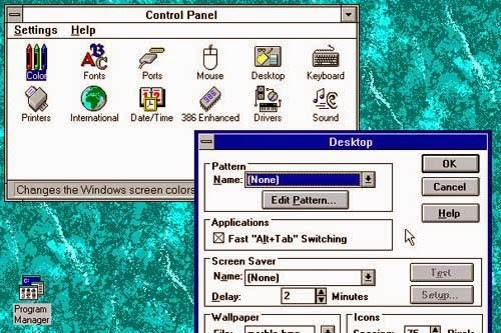
\includegraphics[width=1\textwidth]{figures/Windows31.JPG}}
\caption{tampilan desktop di windows 3.1}
\label{Windows31}
\end{figure}

% Windows 95
\section{windows 95}
\ref{desktop95}
	Windows 95 merukapan sistem operasi hubruda 16-bit/32-biit dan 
	diproduksi oleh microsoft, windows ini di perkenalkan kepada 
	publik pada tanggal 14 agustus 1995. Windows 95 ini adalah produk 
	pertama windows dengan kernel monolotic yg berjalan  -/+  60 tanpa dos 
	dan di dalamnya sudah berisi microsoft office 1995. \cite{petzold1996programming} 
	\subsection{Lima versi windows 95}
		1.windows 95
		2.windows 95 A
		3.windows 95 B
		4.windows 95 B USB
		5.windows 95 C


\begin{figure}[ht]
\centerline{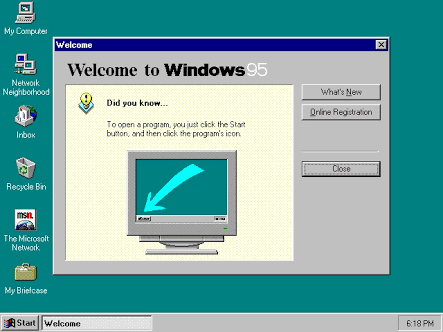
\includegraphics[width=1\textwidth]{figures/desktop95.PNG}}
\caption{tampilan desktop di windows 95.}
\label{desktop95}
\end{figure}

% Windows 98
\section{windows98}
		\ref{Desktopwindows98}
	windows 98 adalah pengembangan dari windows 95 dimana windows 98 diluncurkan agar lebih stabil daripada versi sebelumnya, windows versi 98 ini adalah versi pertama yang dibuat secara spesifik untuk konsumen. pada windows 98 ini memiliki fitur menarik yang disebut \"Deskbar\" fitur ini bisa mengunduh bilah alat desktop(deskbar) dari situs-situs favorit mereka.
	Dalam sebuah artikel dari davis menyebutkan bahwa revisi dari windows 98 adalah pemasangan dan perubahan antarmuka hingga komponen built-in, perangkat tambahan dan multimedia baru dan bagian referensi teknis yang jauh kebih luas. \cite{Davis:1998:W9B:551711}
	\subsection{fitur tambahan dari windows 98}
			Pada windows 98 ini mencakup banyak driver dan dukungan berkas system FAT32.
		Dalam sebuah artikel dari mcfedries menyebutkan bahwa windows 98 memiliki fitur windows terbaru, anda dapat menemukan Internet Explorer 4.0 dan Active Desktop; mengatur Outlook Express untuk surat internet dan surat CompuServer; Instalasi,konfigurasi, dan kostumisasi windows 98 termasuk dua-boot; membuka potensi multimedia windows 98 \cite{mcfedries1998windows}

		\begin{figure}[ht]
		\centerline{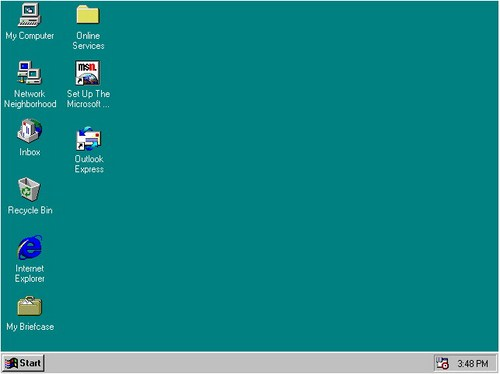
\includegraphics[width=1\textwidth]{figures/Desktopwindows98.JPG}}
		\caption{tampilan desktop windows 98}
		\label{Desktopwindows98}
		\end{figure}

% Windows 2000
\section{windows2000}
	Windows 2000 diluncurkan oleh perusahaan multinasional Microsoft Corporation pada tanggal 17 Februari 2000 di Washington, Amerika Serikat. 
	Dalam sebuah buku yang ditulis oleh Solomon disebutkan bahwa Windows 2000 merupakan flatform dari sistem operasi generasi lanjutan dari windows seri NT4.0 dan menyediakan fitur-fitur lebih tinggi,ekstensi aritmatika yang lebih kuat dan akurat, memiliki instruksi khusus untuk multimedia, serta mendapat dukungan memori yang besar dari chip Intel 64-bit dengan fitur multiprocessing yang luas \cite{solomon2000inside}
	\subsection{tujuan perancangan windows 2000}
		Pada awal pembuatannya, Windows 2000 dirancang untuk memenuhi kebutuhan akan bisnis yang dilakukan melalui dunia maya seperti e-commerce, data dari suatu tempat, proses transaksi online, dan aplikasi yang memiliki performa tinggi.
	\subsection{fokus pengembangan windows 2000}
		Fokus pengembangan Windows 2000 terdapat pada bidang keandalan sistem dan diharapkan sistem operasi baru yang diluncurkan pada saat itu lebih dapat diandalkan dari sistem operasi yang lain.
		Dalam artikel yang ditulis oleh Murphy, tidak adanya standar industri yang ditujukan untuk mengkarakterisasi keandalan sistem menuntut Microsoft agar menambahkan fungsionalitas kerja kedalam sistem operasinya agar lebih dapat diandalkan dan mengurangi persepsi pelanggan mengenai terjadinya bug dan masalah yang akan terjadi dalam penggunaan fungsi dan fitur-fitur baru dasi sistem operasi yang baru ini. Sehingga pelangga akan merasa nyaman dalam menggunakan sistem operasi yang baru ini \cite{murphy2000windows} 

% Windows 2003 server
\section{windows 2003 server}
\ref{windows2003server}
	windows 2003 adalah pembaruan dari windows 2000 server yang menggabungkan kompatibilitas dan fitur-fitur lainnya dari windows XP, alasan windows 2003 ini menggunakan metode kompatibilitas agar aplikasi lama dapat bekerja dengan stabiLitas yang besar, semua itu dibuat kompatibel dengan jaringan yang berbasis windows NT 4.0 . pada windows 2003 ini menawarkan berbagai fitur keamanan baru, seperti \"Manage Your Wizard\".
	dalam sebuah artikel yang ditulis oleh Litch Field menyebutkan bahwa windows 2003 dirancang agar aman diluar kontak. Sebagian dari keamanan diadopsi oleh microsoft untuk versi windows terbaru dengan tujuan mengurangi resiko yang ditimbulan oleh kerentangan buffer offerflow \cite{litchfield2003defeating}
	\subsection{edisi windows server 2003}
		windows server 2003 menggunakan kernel windows NT versi 5.2 
		windows server 2003 tersedia dalam lima buah edisi:
		1.windows server 2003 standart edition
 		2.windows server enterprise edition (32bit dan 64bit)
		3.windows server datacenter edition
		4.windows server small business server
		5.windows strorage server 2003


\begin{figure}[ht]
\centerline{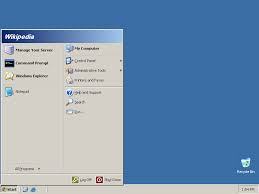
\includegraphics[width=1\textwidth]{figures/windows2003server.JPG}}
\caption{tampilan desktop di windows 2003 server}
\label{windows2003server}
\end{figure}
% Windows XP
	\section{Windows XP}
		Windows XP dirilis setelah Windows 2000 dan Windows Me (millenium edition), Windows XP sebelumnya dikenal dengan sebutan sandi Whistler. Dan pertama kali dipublikasikan tanggal 25oktober 2001. Windows XP adalah kependekan dari Windows Experience yang artinys pengalaman. Windows XP mempunyai daya tarik tersendiri karena Windows XP merupakan Windows pertama yang dibangun diatas kernel dan arsitektur Windows NT.\cite{pogue2002windows}\ref{windowsxp}
		\subsection{jenis Windows XP}
			1.Windows XP Professional
			2.Windows XP Home Edition
			3.Windows XP Media Center Edition
			4.Windows XP Tablet PC Edition
			5.Windows XP Starter Edition
			6.Windows XP Professional X64 Edition
			7.Windows XP Professional 64-Bit Edition for Itanium
		\subsection{fiture dan peningkatan}
			Windows XP menggabungkan home line dengan corporate line nya sehingga menjadi sistem terpadu yang sangat baik. Windows XP memiliki kestabilan dan efisieni yang telah melebihi Windows 98, Windows ME, dan Windows 2000 professional, hal ini disebabkan Windows XP memiliki software untuk menghindari yang disebut dengan \"neraka DLL\" atau \"DLL HELL\".
			\subsubsection{Stabilitas}
				Jika suatu program rusak, program itu tidak akan mengganggu memori yang digunakan program lain. Inilah tindakan tindakan microsoft untuk membuat PC stabil:
		 			a. Perlindungan file sistem
		 			b. Manajemen lebih berhati hati
		 			c. Sistem otomatis update
			\subsubsection{Perubahan tampilan}
				Windows XP telihat lebih bagus dengan taskbar dan Windows berwarna biru terang. juga ikon memiliki tampilan gelap 3D
			\subsubsection{Gmabar, Musik, dan Film}
				Windows XP mendapatkan penghargaan karena telah memasukan kamera digital ke dalam PC.
			\subsubsection{Dukungan terhadap sistem domain Active Directory} 
				Active Directory merupakan suatu sistem yang dapat diatur dari satu tempat saja, yaitu dari sistem yang menjalankan sistem itu sendiri. Fitur ini dapat meneyderhanakan 	proses autentikasi di perusahaan perusahaan besar.
			\subsubsection{Peningkatan pengaturan kontrol akses}
				Windows XP ditujukan untuk penggunaan korporasi,sehingga telah dilengkapi dengan pengaturan kontrol akses. Fitur ini digunakan untuk membatasi akses yang tidak memiliki izin akses terhadap objek tertentu.
			\subsubsection{Mendukung sistem bekas terenskripsi}
				Fiture ini digunakan untuk melindungi data data penting sehingga tidak dapat dibuka orang lain, kecuali dengan membuka kodenya.

\begin{figure}[ht]
\centerline{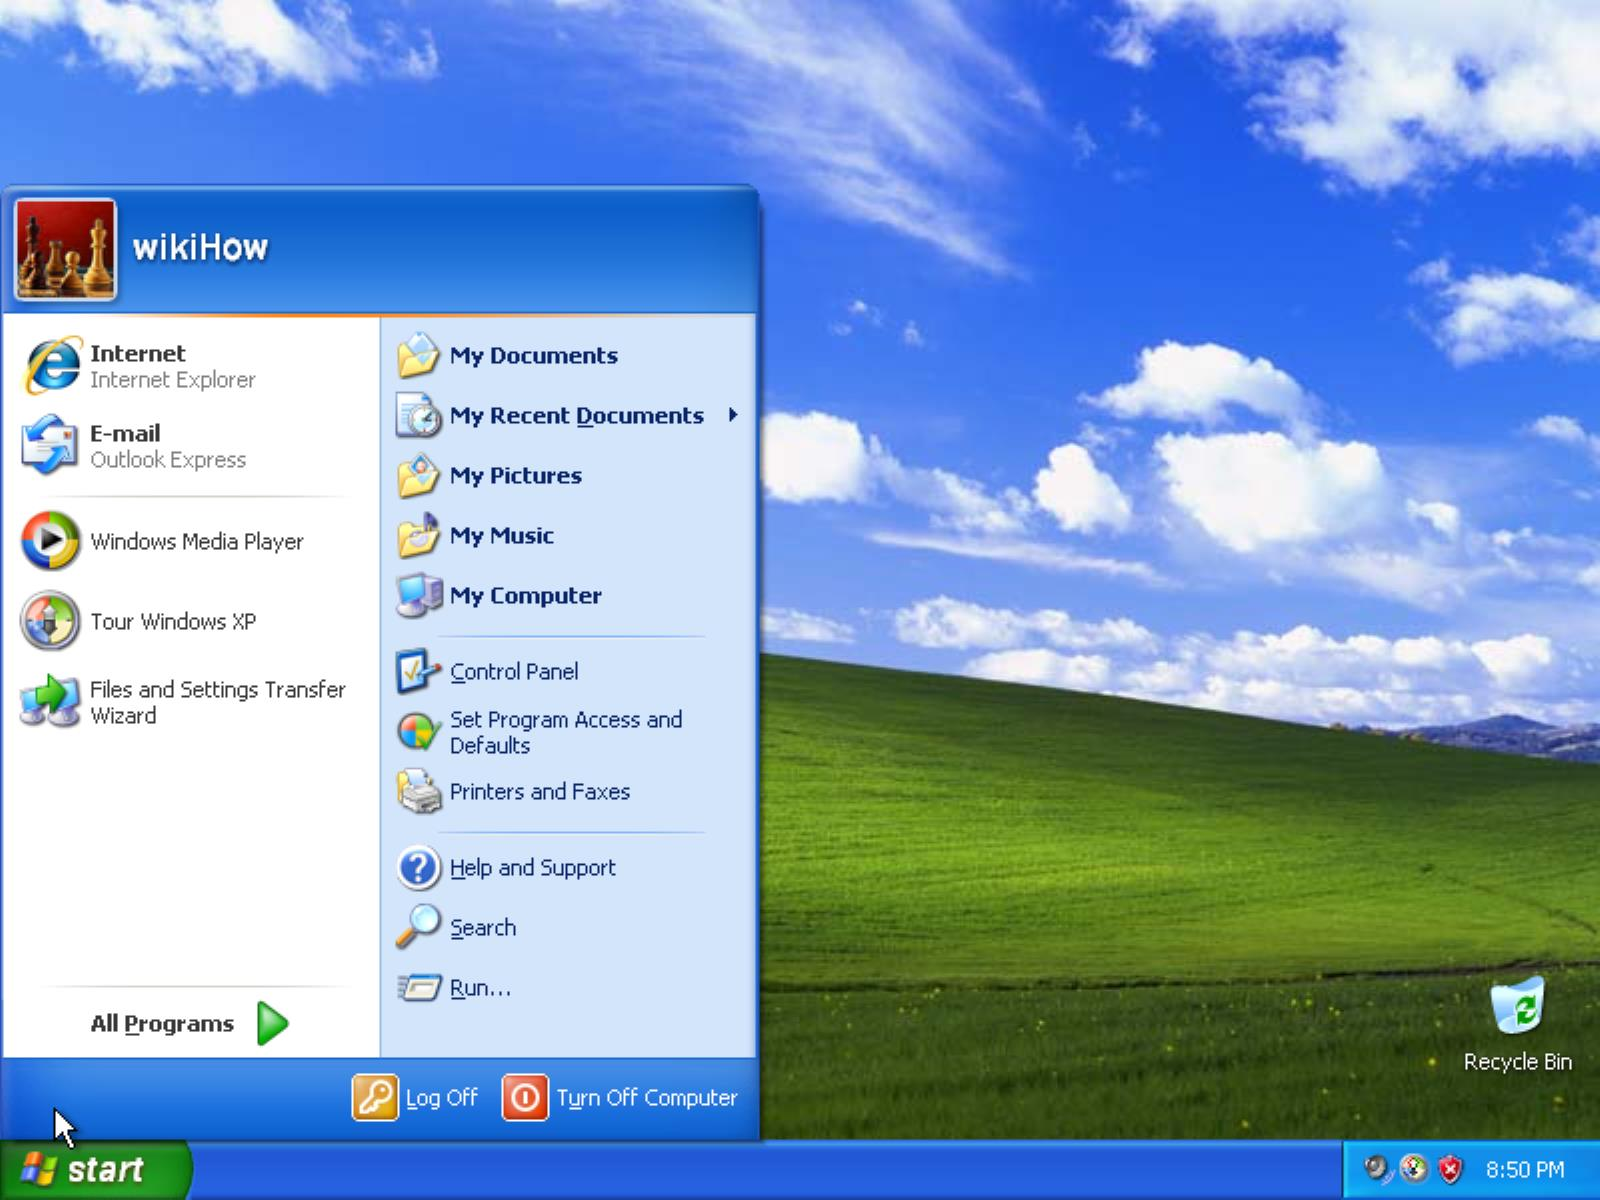
\includegraphics[width=1\textwidth]{figures/windowsxp.JPG}}
\caption{tampilan desktop di windows XP}
\label{windowsxp}
\end{figure}
% Windows Vista
	\section{Sejarah Windows Vista}
\ref{vista1}
		Windows Vista adalah sistem operasi berbasis dari Microsoft pada PC, Windows Vista dirilis pada tanggal 22 Juli 2005, Windows Vista ini lebih dikenal dengan Longhorn
	\subsection{Kelebihan dan Kekurangan Windows Vista}  \cite{russinovich2009windows}
		\subsubsection{Kelebihan:}
			1. Kualitas warna yang lebih tinggi, sehingga GUI (Grhapic User Interface) lebih bagus
			2. Bisa membaca RAM up to 16 GB
			3. Mendukung direct X 10
			4. Lebih cepat menjalankan program
			5. Banyak fitur baru yang tidak ada dalam versi sebelumnya
			6. Pencarian file lebih mudah 
		\subsubsection{Kekurangan:}
			1. Terdapat beberapa aplikasi yang belum support
			2. Terlalu banyak varian seri
	\subsection{Spesifikasi Hardware}
		\subsubsection{Minimum}
			Processor 800 Mhz(Pentium III atau Athlon)
			RAM 512 Mb
			Hard disk 40 Gb
			Graphic card bebas
		\subsubsection{Medium}
			Processor 2Ghz(Pentium 4 2,6 Ghz, Athlon XP 2800+ dll)
			RAM 1024 Mb
			Hard disk Sata 80 Gb
			Graphic card Direct x 9.0 (128 - 256 MB)
		\subsubsection{High}
			Processor 3 Ghz atau lebih, Processor Dual Core
			RAM 2048 Mb DDR II
			Hard disk Sata 120 Gb
			Graphic card Pixel Shader 2/3. (>256 MB)


\begin{figure}[ht]
\centerline{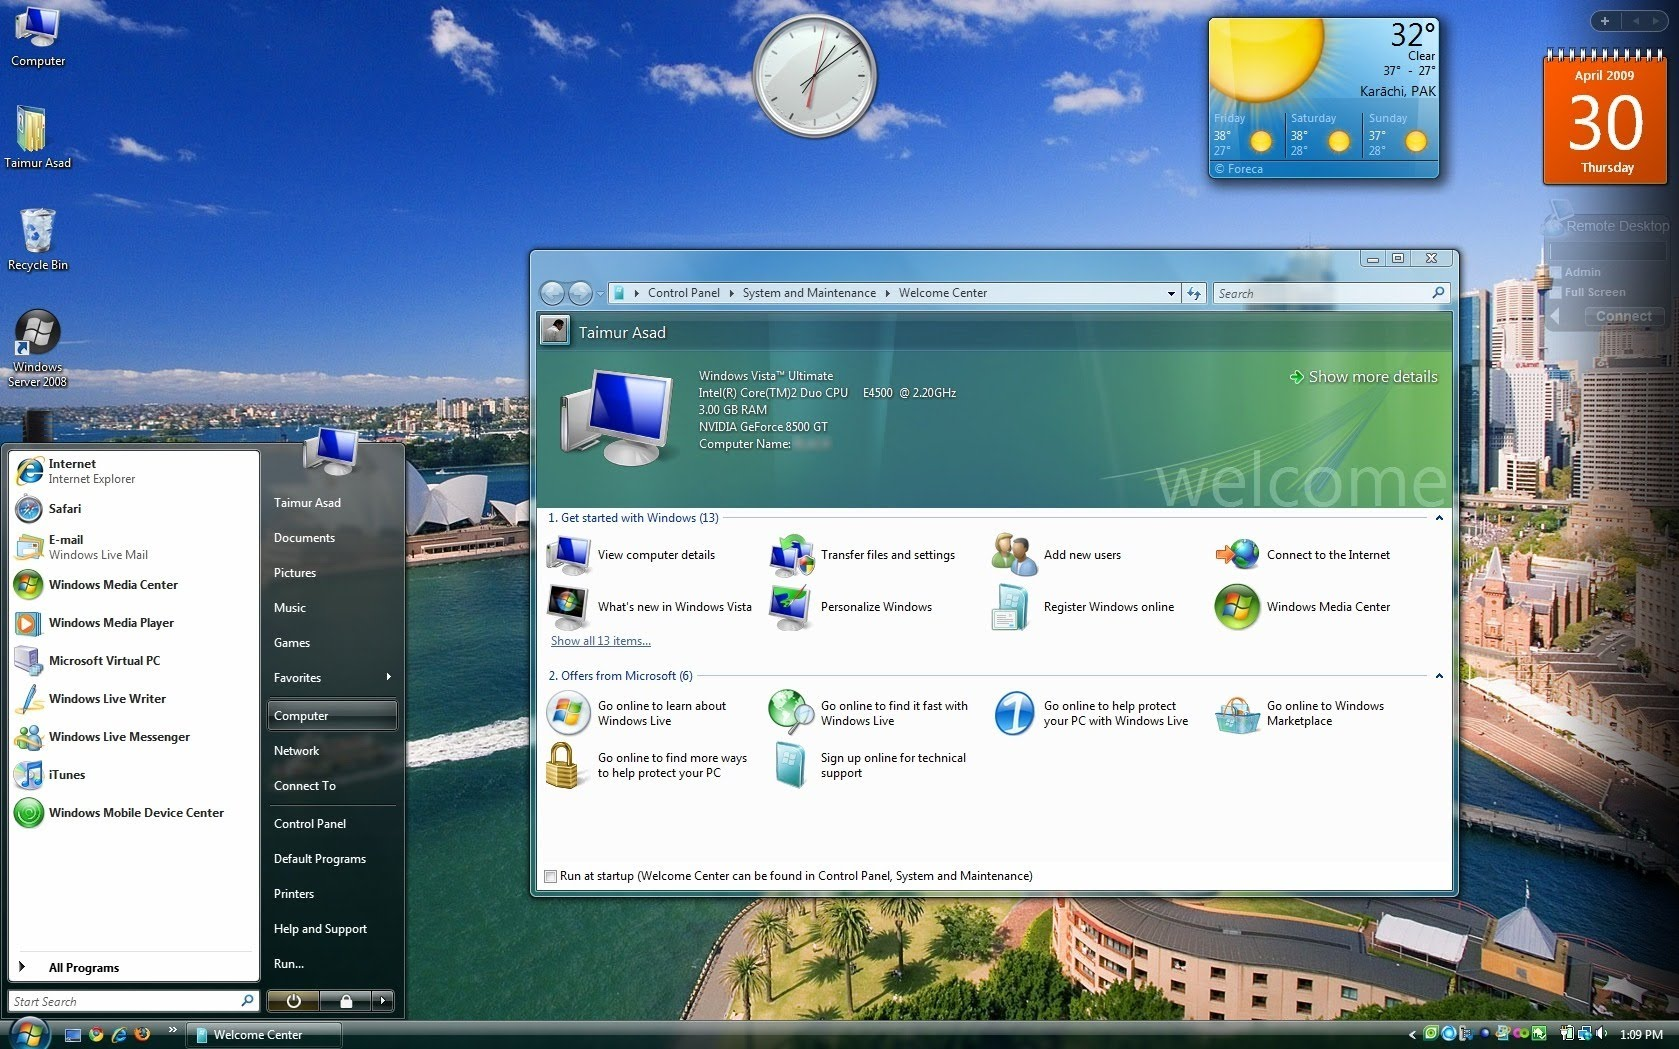
\includegraphics[width=1\textwidth]{figures/vista1.JPG}}
\caption{tampilan desktop di windows vista}
\label{vista1}
\end{figure}


% Windows 7
	\section{windows 7}
\ref{desktop7}
		Ada fitur fitur baru di windows 7 yang memberikan tantangan untuk memori
		dan juga menawarkan informasii yang dapat dipulihkan dan di ambil dari
		gambar,file,dan makalah. Fitur baru di windows 7 ini di kembangkan 
		metode analisis memori sesuai fitur masing masing. Metode ini
		berlandasan pada struktur data windows yangbernama dengan kernel
		processor. Proses yang berjalan pada windows ini ada 2 yaitu windows 7 
		7 dan 64-bit dan 32-bit windows 7
		\subsection{pendahuluan}
			Memori komputer sangat lah berguna sebagai sumber daya juga menawarkan
			Semua sistem operasi sepenuhnya dijalankan COROM, dan hampir semua
			semua informasi berhaga ada di memori komputer.
		\subsection{windows 7 edisi}
			1.windows 7 starter.
			2.windows 7 prefessional.
			3.windows 7 home basic.
			4.windows 7 enterprise.
			5.windows 7 ultimate.
			6.windows 7 home premium.
		\subsection{analisi windows 7 dan memori}
			\subsubsection{Gambaran dari windows 7}
				Ada pun perbadingan dengan widows 2000 dan windows xp, fitur windows 7 
				dijelaskan sebangai berikut. Strktur KPCR terletak di virtual OxFFDFFOOO
				di windows 7 KPCR dan KPCRB berada tidak terletak di alamat ini karna
				alamat struktur KPCR tidak dapat di temukan oleh lokasi stirng biner 
				00fdfff0fldff dalam gambar memo.(2) masing-masing objek karel adalah 
				prefxed oleh struktur objek header di windows 2000, dalam object header
				struktur windows 7, type variabel adalah bukan dengan variabel 
				Typelndex.(3)log peristiwa jendela telah berubah di windows 7. Fornat 
				yang bary untuk event log dan perpanjangan baru adalah \"EVTX\" 
				dan terletak di \verb|"C: \Windows\System32\winevvt\Logs\"|
		\subsubsection{alamat terjemahan}
			Karena alamat di memori umumnya di simpan sebagai alamat virtual,dan 
			alamat fisik digunakan untuk analasisi memori maka pentung untuk 
			menerjemahkan alamat virtual tersebut ke alamat fisik dengan 
			mempelajari terjemahan alamat prosesor intel. Proses terjemahan :  
			(1) Akuisisi struktur KPCR, variabel CurrentPrcb berikut nya ke 
			variable Self. Nilai variable diri diteruskan ke variavle currentPrcb 
			subsection(Registri)
			Registri windows adalah terdiri dari sejumlah fles biner yang berbeda 
			disebut juga dengan gatal-gatal pada disk. Sarang fles adalah unit 
			alokasi yang disebut blok. Blok utama dari sarang adalah blok dasar.

\cite{zhang2010exploratory} 

\begin{figure}[ht]
\centerline{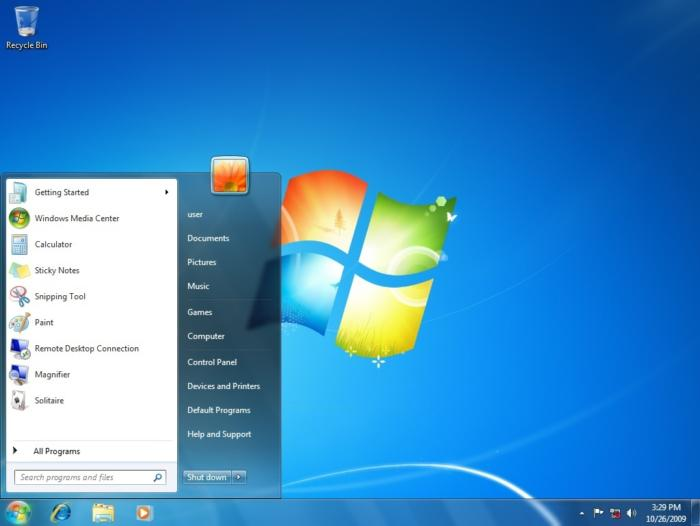
\includegraphics[width=1\textwidth]{figures/desktop7.JPG}}
\caption{tampilan desktop di windows 7}
\label{desktop7}
\end{figure}

% Windows server 2008
	\section{Windows Server 2008}
\ref{windowsserver2008}
	Windows Server 2008 merupakan sebuah sistem operasi yang powerful untuk PC server dan jaringan komputer. Windows Server 2008 diterbitkan sekitar 9 tahun yang lalu, tepatnya bulan februari tahun 2008.\cite{wahyono2009practice}
	\subsection{Sejarah dan Perkembangan}
		Sistem operasi Windows NT masih ada kaitannya dengan perkembangan Windows Server. Tahun 2007 Windows Server yang dikenal dengan nama \" Windows Server Codenamed Longhorn\" dikembangkan oleh microsoft. Longhorn diciptakan untuk menggantikan Windows Server 2003. Sesuai dengan keputusan Bill Gates tanggal 15 mei 2007 Windows Server Longhorn berubah menjadi Windows Server 2008.
	\subsection{Spesifikasi Sistem}
		\subsubsection{Prosesor}
		Minimal 1 GHz (X86 Processor) atau 1.4 GHz (x64 Processor)
		\subsubsection{Memori}
		Minimal yang dibutuhkan adalah 512 MB RAM. Maksimum untuk 32-Bit adalah 4 GB(standar) atau 64 GB(Enterpise dan Datacenter). Untuk yang 64-Bit Maksimumnya adalah 8 GB (Foundation), 32 GB (Standar), dan 2 TB (Enterpise, Datacenter, dan Itanium)
		\subsubsection{Hardisk}
		Minimum untuk 32-Bit adalah 20 GB dan untuk 64-Bit adalah 32 GB.
		\subsubsection{Display}
		Minimal Super VGA (800 x 600). Tetapi untuk pengalaman yang lebih baik menggunakan resolusi yang lebih tinggi.
	\subsection{Fitur penting}
	Windows Server 2008 mempunyai arsitektur dan fungsional lebih maju dibandingkan para pendahulunya. Dan juga memiliki kelibihin instalasi yang lebih mudah, diagnosis kesalahan, dan keamanan yang tangguh.

\begin{figure}[ht]
\centerline{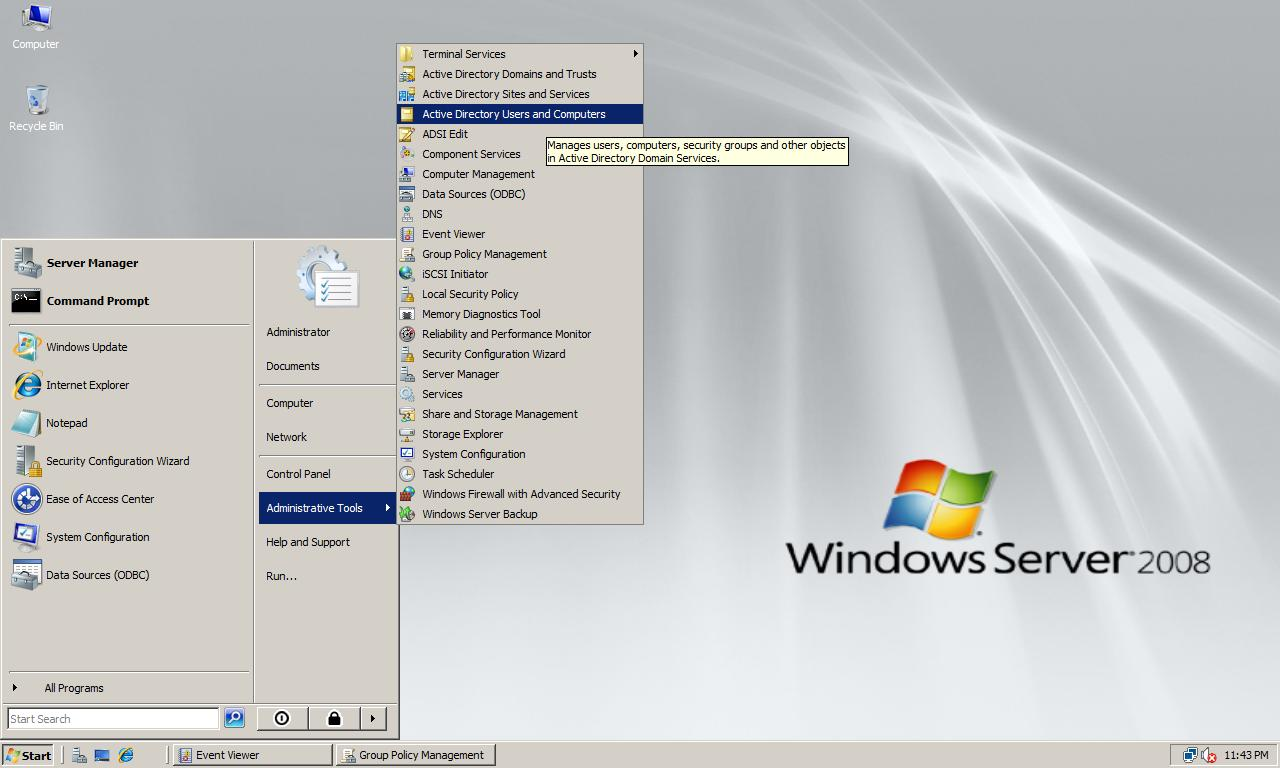
\includegraphics[width=1\textwidth]{figures/windowsserver2008.JPG}}
\caption{tampilan desktop di windows server 2008}
\label{windowsserver2008}
\end{figure}
% Windows 8
	\section{windows 8}
		\ref{tampilanwindows8} windows 8 diluncurkan oleh microsoft pada tahun 2012. dengan dirilisnya windows 8 ini mengubah format file hibernasi, memecah semua alat analisis yang ada.
		Dalam artikel yang ditulis oleh sylve mengemukakan bahwa pada saat itu matthieu suiche mempelajari format file hibernasi windows modern, pada bulan mei 2016 suiche mengumumkan versi beta Hibr2Bin yang mendukung file hibernasi windows 8. Hibr2Bin adalah alat yang mengubah file hibernasi windows menjadi gambar memori mentah sehingga bisa dianalisis dengan alat analisis memori yang secara native tidak mendukung penguraidan file hibernasi. Hibr2Bin diperbarui dan rilis secara terbuka pada akhir september 2016. \cite{sylve2017modern}
		\subsection{Fitur tambahan pada windows 8}
			Seperti yang di kutip pada artikel wahyu asri, windows 8 memiliki fitur tambahan yang memiliki kelebihan sebagai berikut :
			1. Optimalisasi untuk layar sentuh
			2. mendukung chip ARM
			3. toko aplikasi windows store
			4. mendukung NFC (Near Field Communication)
			5. waktu boot yang singkat
			6. Internet Explore 10
			7. Security lebih baik
			8. windows 8 tidak membutuhkan upgrade PC \cite{wahyu8review}

\begin{figure}[ht]
\centerline{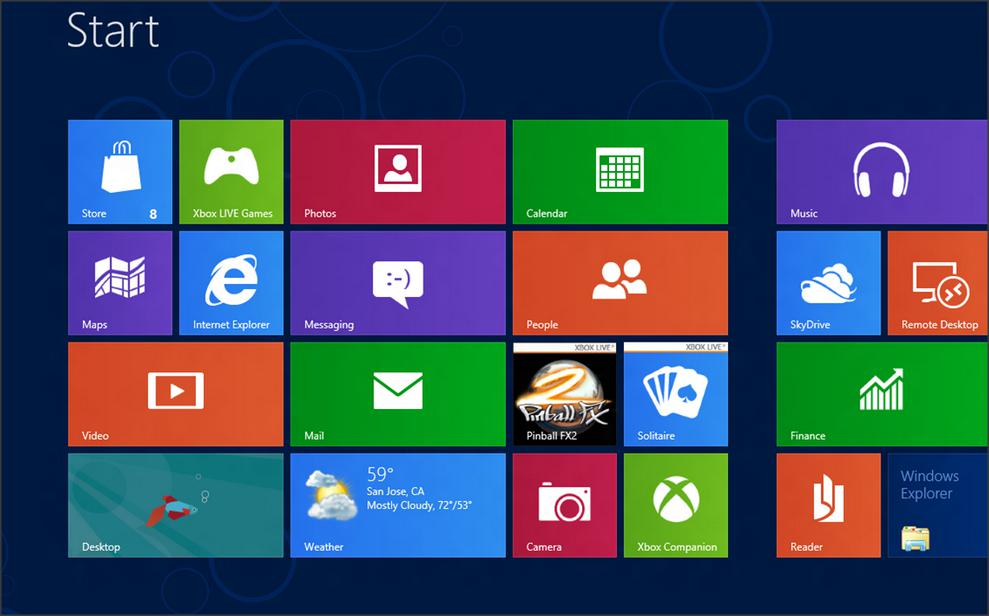
\includegraphics[width=1\textwidth]{figures/tampilanwindows8.JPG}}
\caption{tampilan desktop di windows 8.}
\label{tampilanwindows8}
\end{figure}


% Windows 2012 server
	\section{windows 2012 server}
		\ref{windows12} windows 2012 server merupakan sistem operasi penyempuraan dari windows sebelumnya yaitu windows 2008 R2. Windows 2012 ini merupakan versi server windows 8, pada windows 2012 ini, 
		menawarkan berbagai fitur-fitur baru dan juga peningkatan-peningkatan pada windows server. Windows ini resmi diperkenalkan pada november 2012. Tidak seperti windows 2008 R2 windows 
		2012 server ini tidak memiliki dukungan komputer yang berbasis itanium dan pada windows 2012 server ini banyak menekankan penggunaan cloud pribadi, sehingga pengguna dapat 
		mengaplikasikan dengan mudah. pada windows 2012 ini juga membantu memudahkan pengguna untuk menginstal mesin virtualnya secara efisien. disamping itu windows 2012 ini memiliki beberapa
		fitur untuk memperbaiki windows 2008 R2. dengan adanya semua fitur yang ada pada windows 2012 tersebut pengguna akan dapat mempelajari segala sesuatu mulai dari instalisasi, 
		keamanan, konfigurasi otomasi, pemantauan dan lain sebagainya yang dimuat dalam format resep praktis\cite{carvalho2012windows}
		\subsection{edisi windows server 2012}
			1.windows server 2012 foundation
			2.windows server 2012 essantiasis
			3.windows server 2012 standard
			4.windows server 2012 datacenter
			5.windows multipoint server 2012

\begin{figure}[ht]
\centerline{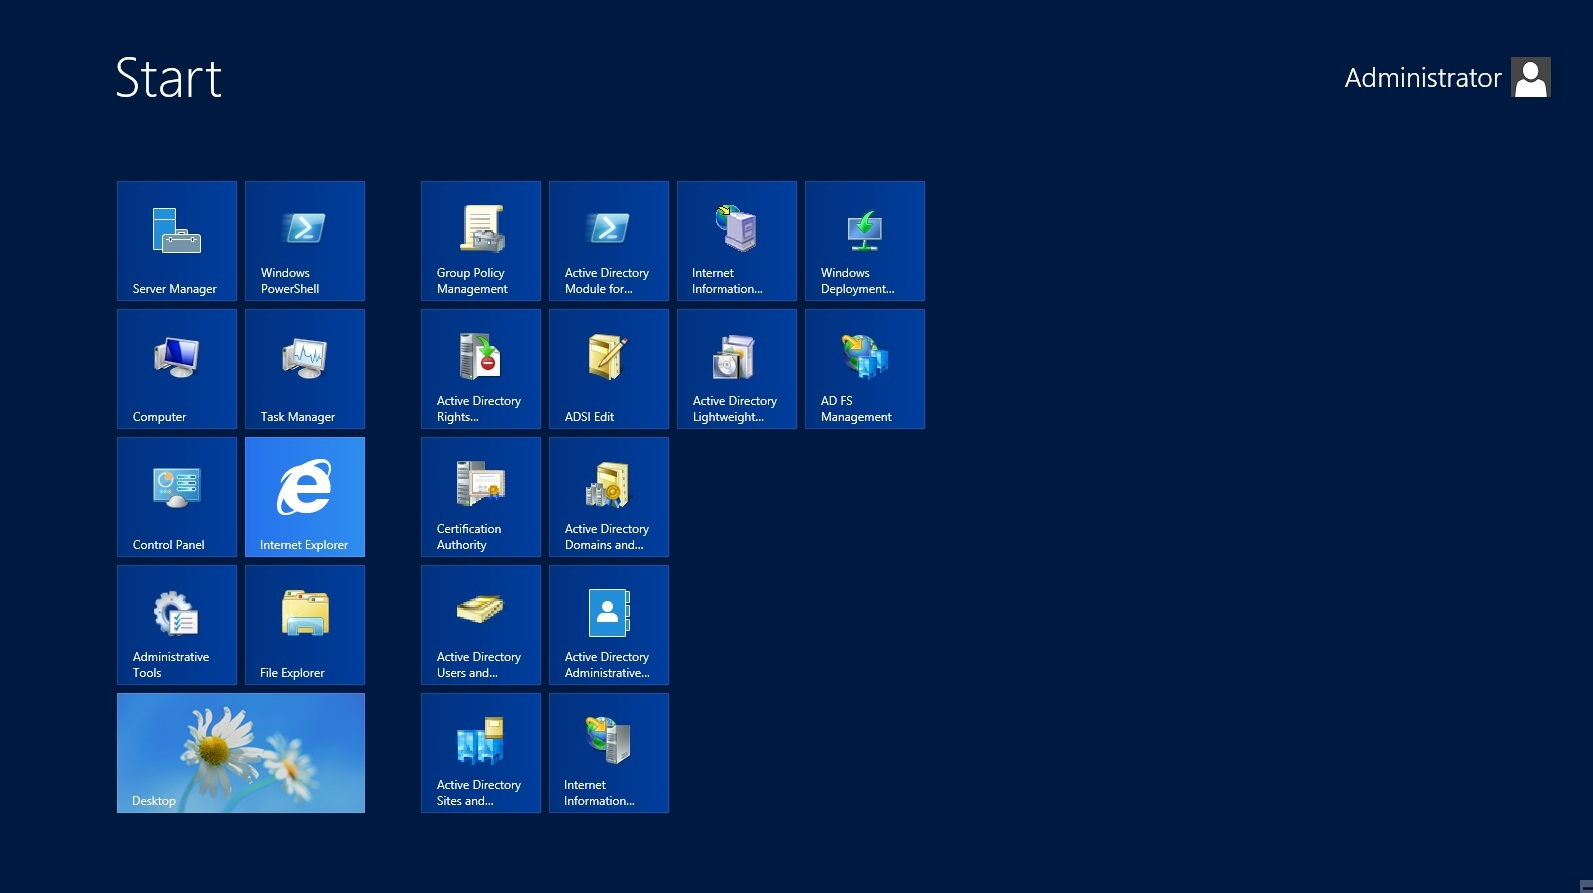
\includegraphics[width=1\textwidth]{figures/windows12.JPG}}
\caption{tampilan desktop di windows server 2012}
\label{windows12}
\end{figure}

	
% Windows 10
	\section{windows10}
		Windows 10 merupakan salah satu sistem operasi yang dirilis oleh perusahaan multinasional Microsoft Corporation pada tanggal 29 juli 2015. windows 10 dikenal sebagai suatu sistem 
		operasi yang selalu menerima pembaharuan terhadap fitur fitur yaang ada didalamnya. Pada awal peluncurannya, Microsoft Corporation mengadakan sebuah kampanye periklanan yang 
		mengenai perilisan windows 10 yang memiliki tema \"Upgrade Your World\". Dalam iklan tersebut, perusahaan ini menggunakan tagline \"Cara Yang Lebih Manusiawi Untuk Diakses\" berikut gambar dari windows 10 \ref{tampilanwindows10}
		\subsection{keunggulan dan fitur fitur windows 10}
			Dalam sebuah buku yang ditulis oleh JJ. Foster menyebutkan sistem operasi versi terbaru dari Microsoft ini mampu membangun keselarasan pengalaman dan fungsionalitas pengguna 
			dalam perbedaan kelas perangkat \cite{foster2001data} 
			Pada fitur windows 10 terdapat Windows Store yang berfungsi sebagai wadah untuk mendownload aplikasi. gambar ditampilkan sebagai berikut\ref{Store}, Groove Music sebagai 
			aplikasi pemutar musik. gambar ditampilkan sebagai berikut\ref{Groove}, dan Films dan Tv sebagai aplikasi pemutar video dan film. Gambar ditampilkan sebagai berikut\ref{filmstv}. 
			Tidak hanya itu, Windows 10 juga menyedikan fitur Xbox yang memungkinkan para pengguna untuk menjelajah perpustakaan permainan. Gambar ditampilkan sebagai berikut\ref{Xbox}
		\subsection{fitur yang dihapus}
			Akan tetapi, ada juga fitur yang tidak dilanjutkan pengembangan bahkan dihapus saat diupgrade dari versi sebelumnyl.a. Fitur tersebut adalah:
			-Windows Media Center
			-Aplikasi makanan dan minuman
			-Aplikasi kesehatan
			-dan aplikasi travel/perjalanan.

\begin{figure}[ht]
\centerline{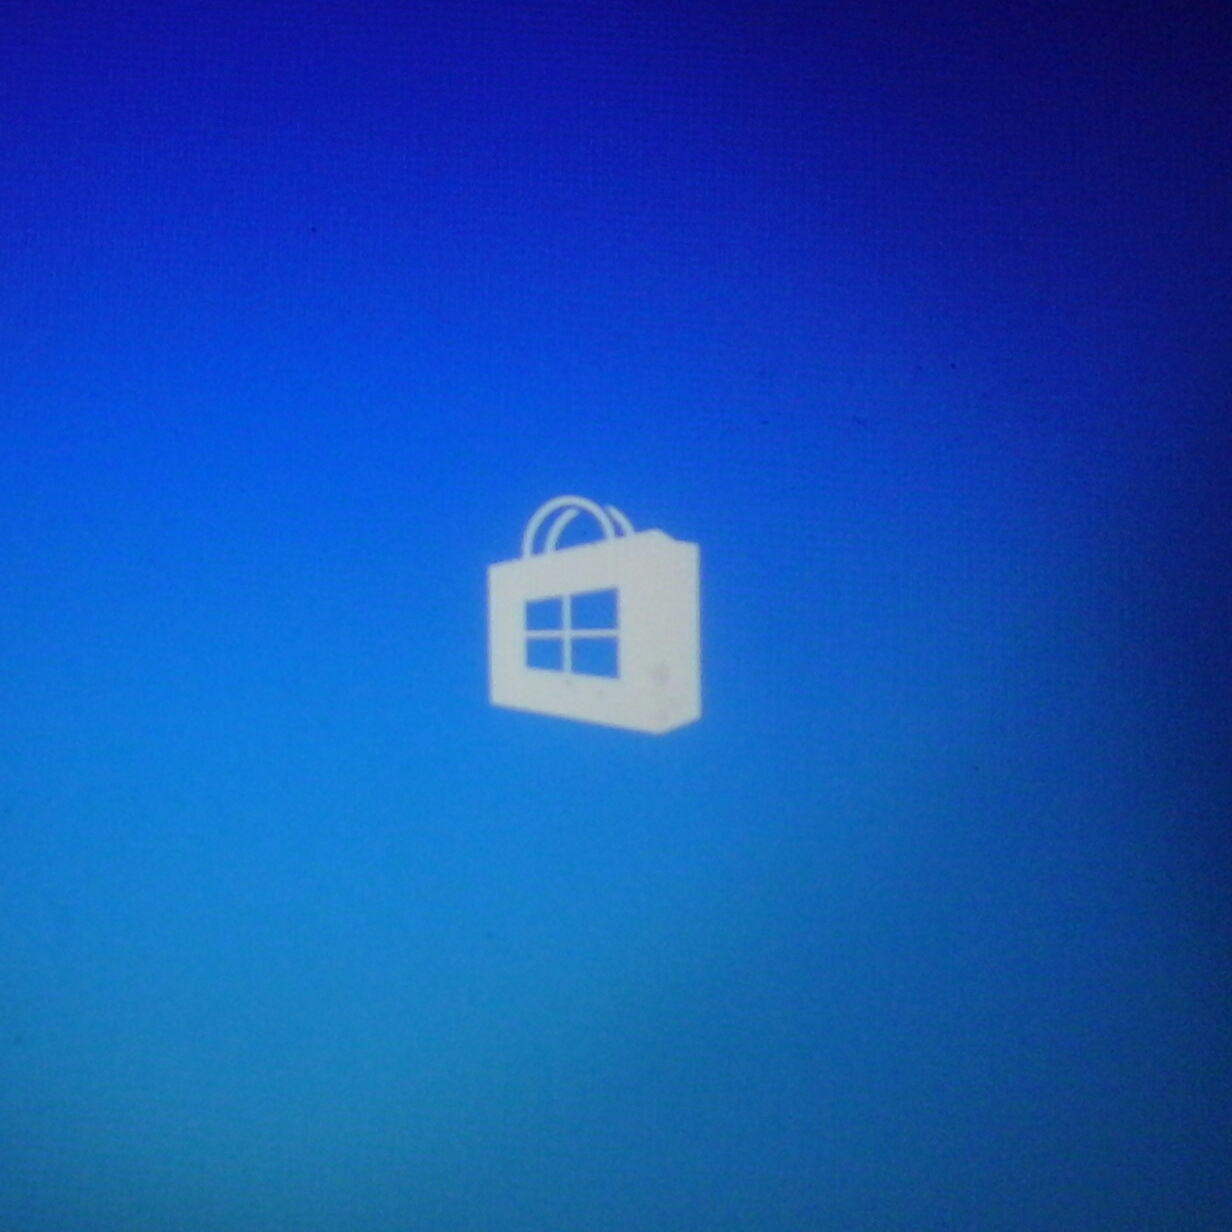
\includegraphics[width=1\textwidth]{figures/Store.JPG}}
\caption{tampilan Store}
\label{Store}
\end{figure}

\begin{figure}[ht]
\centerline{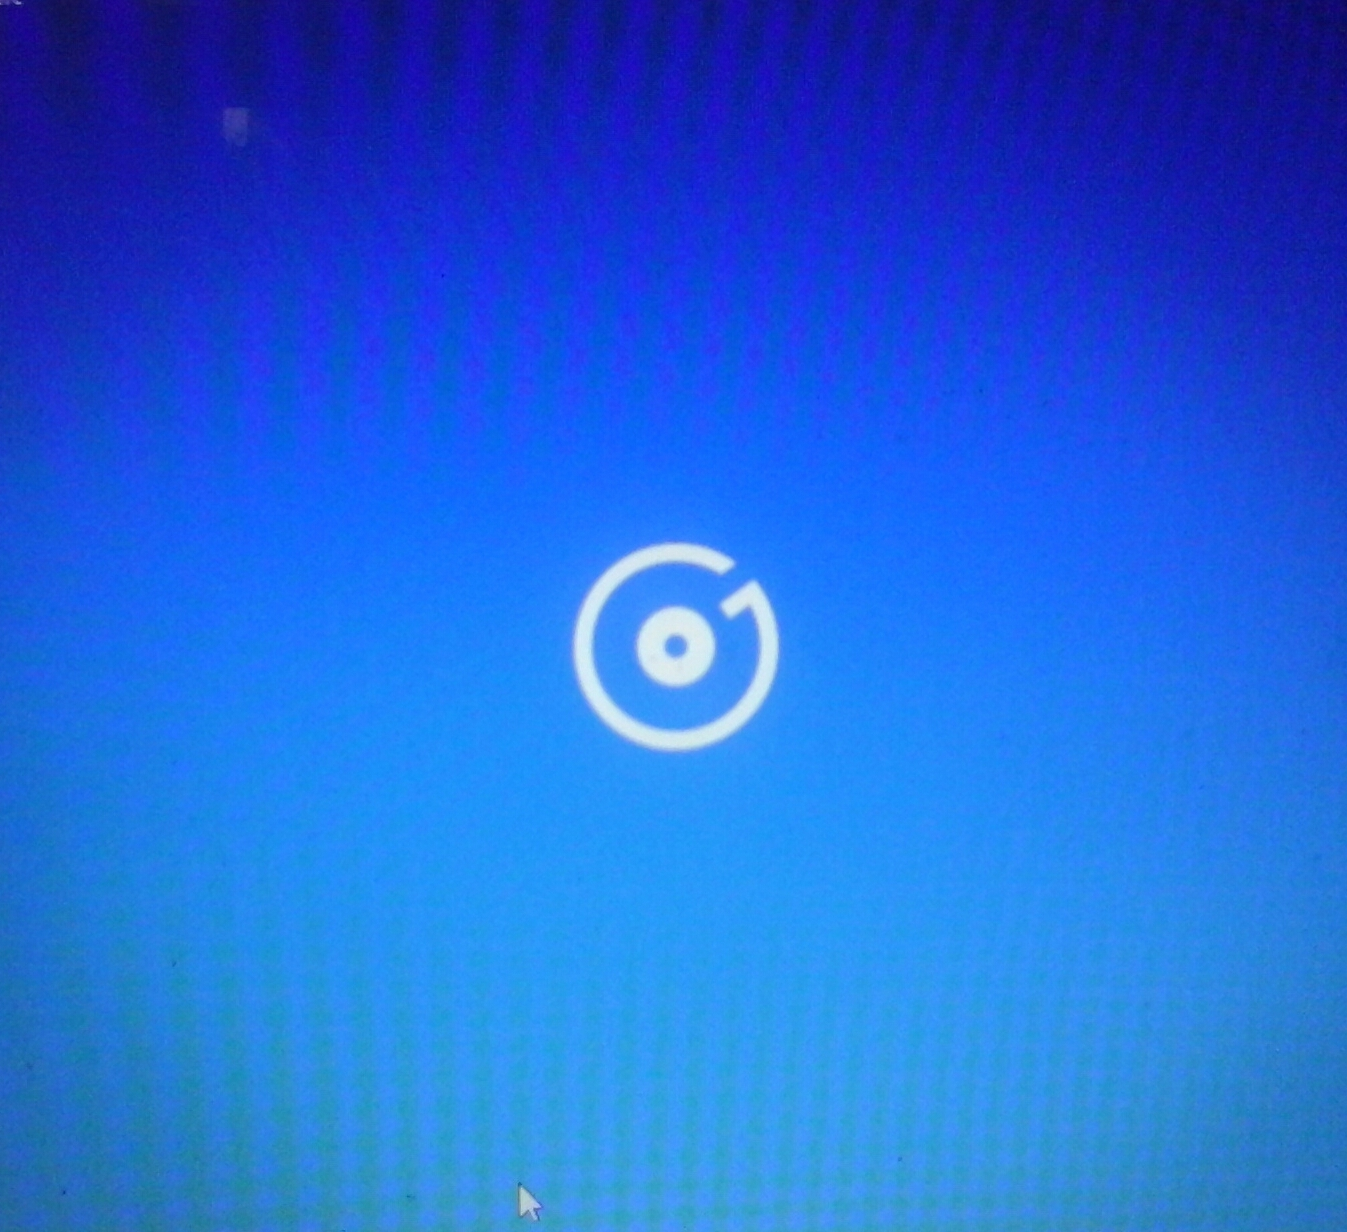
\includegraphics[width=1\textwidth]{figures/Groove.JPG}}
\caption{tampilan Groove}
\label{Groove}
\end{figure}

\begin{figure}[ht]
\centerline{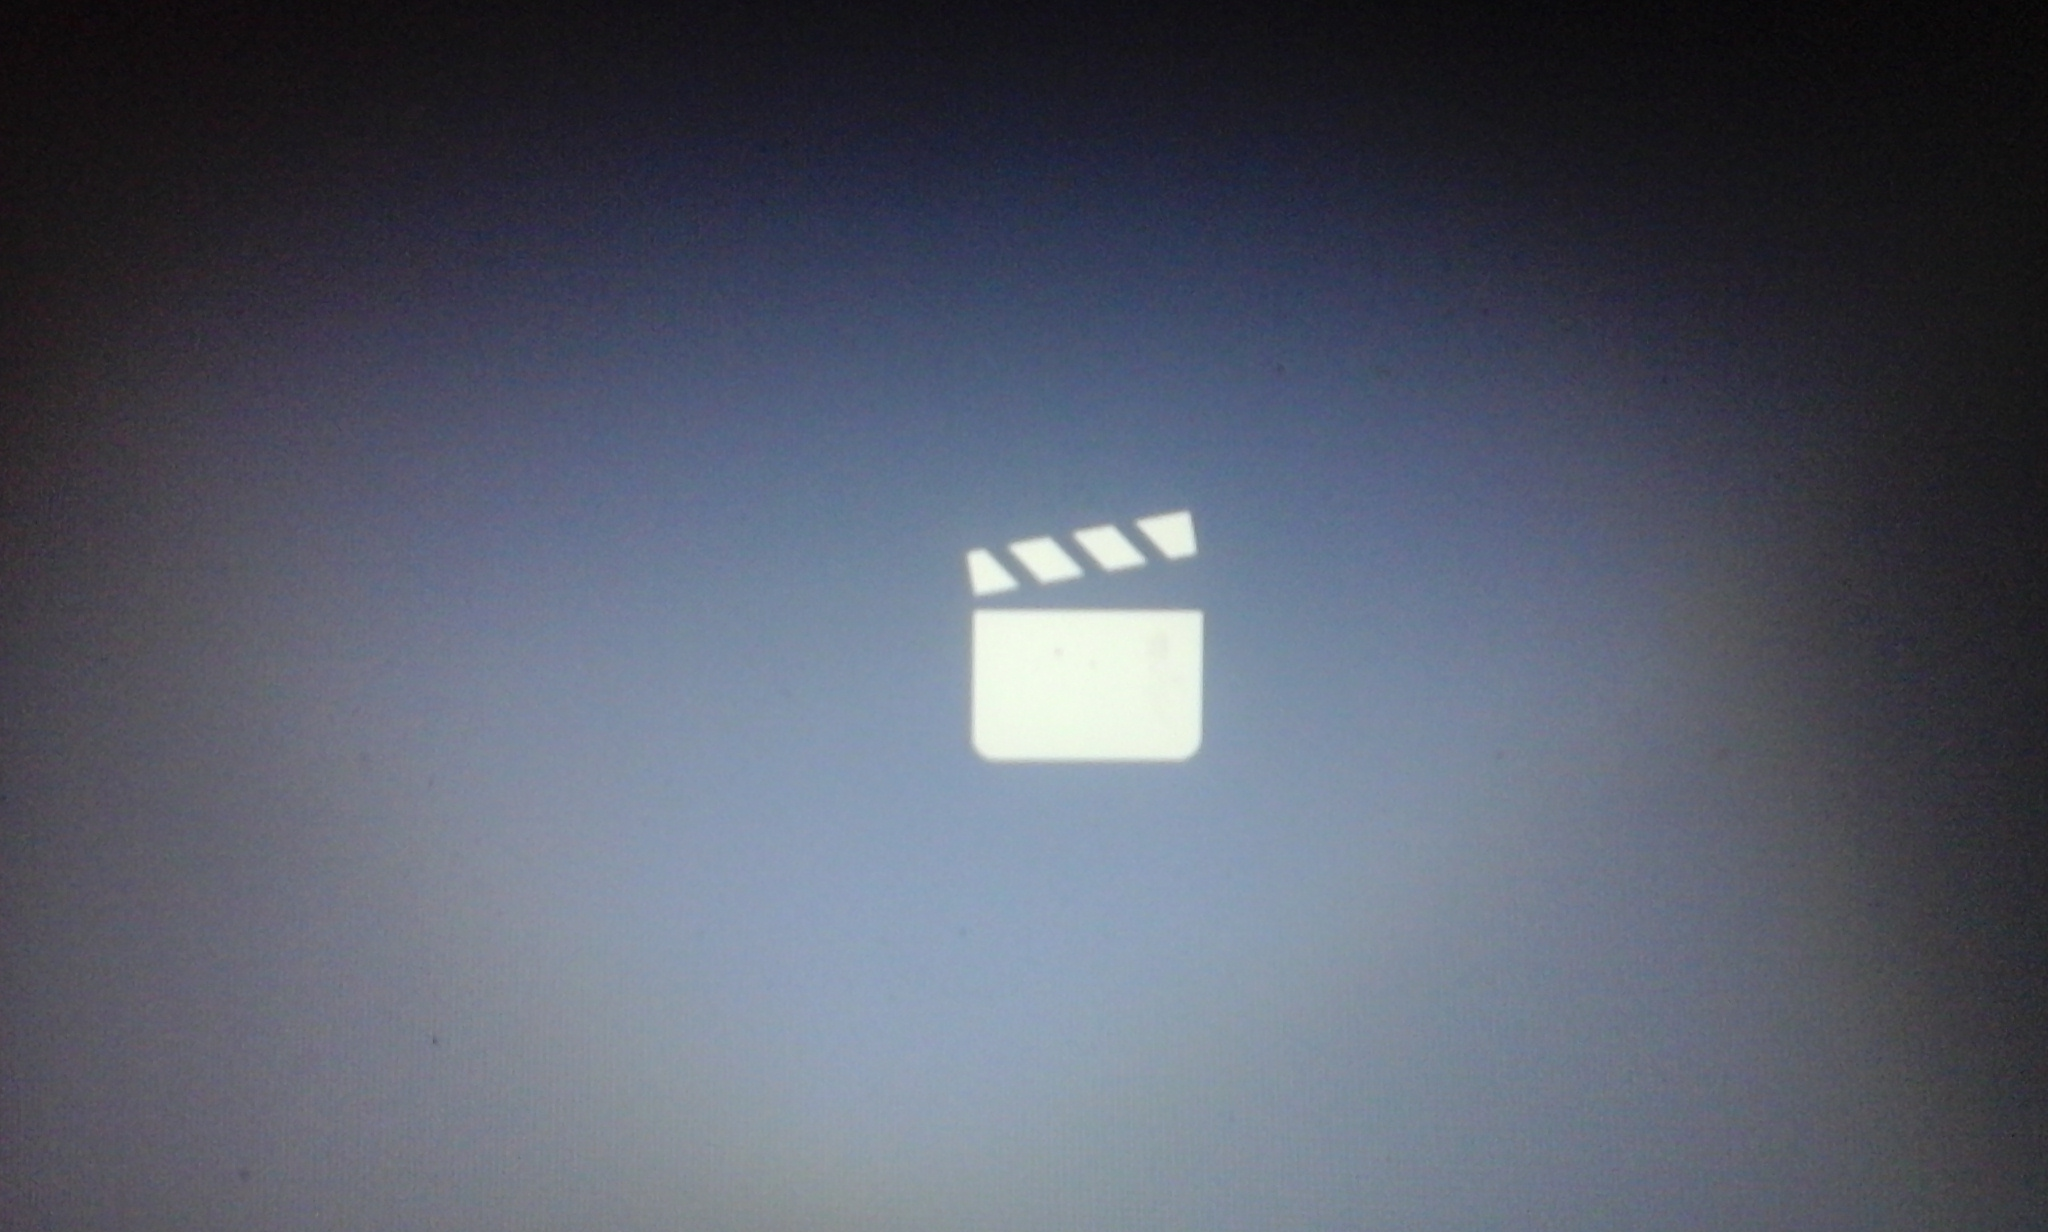
\includegraphics[width=1\textwidth]{figures/filmstv.jpg}}
\caption{tampilan Films Tv}
\label{filmstv}
\end{figure}

\begin{figure}[ht]
\centerline{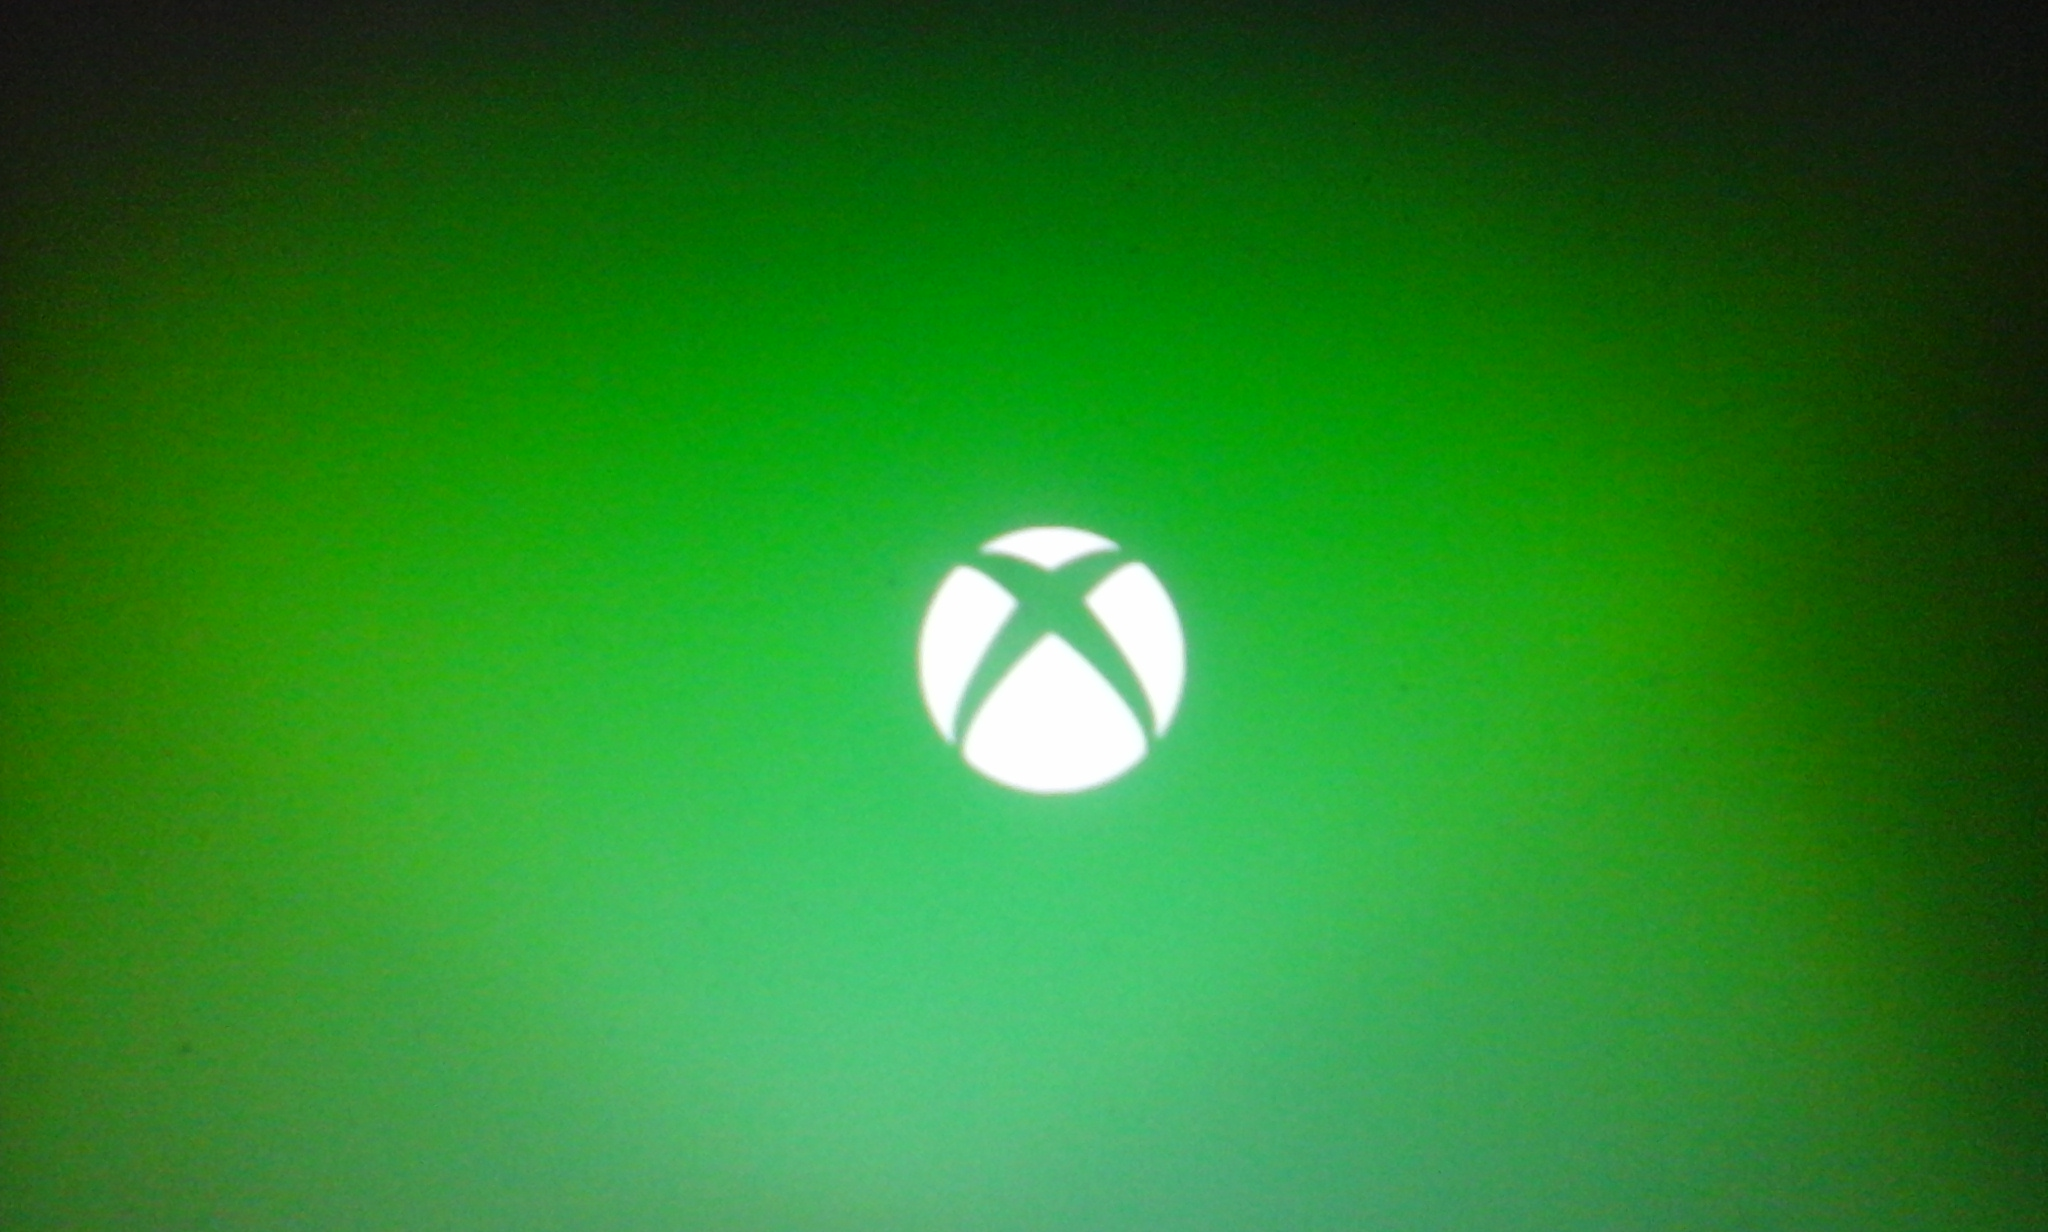
\includegraphics[width=1\textwidth]{figures/Xbox.JPG}}
\caption{tampilan Xbox}
\label{Xbox}
\end{figure}

\begin{figure}[ht]
\centerline{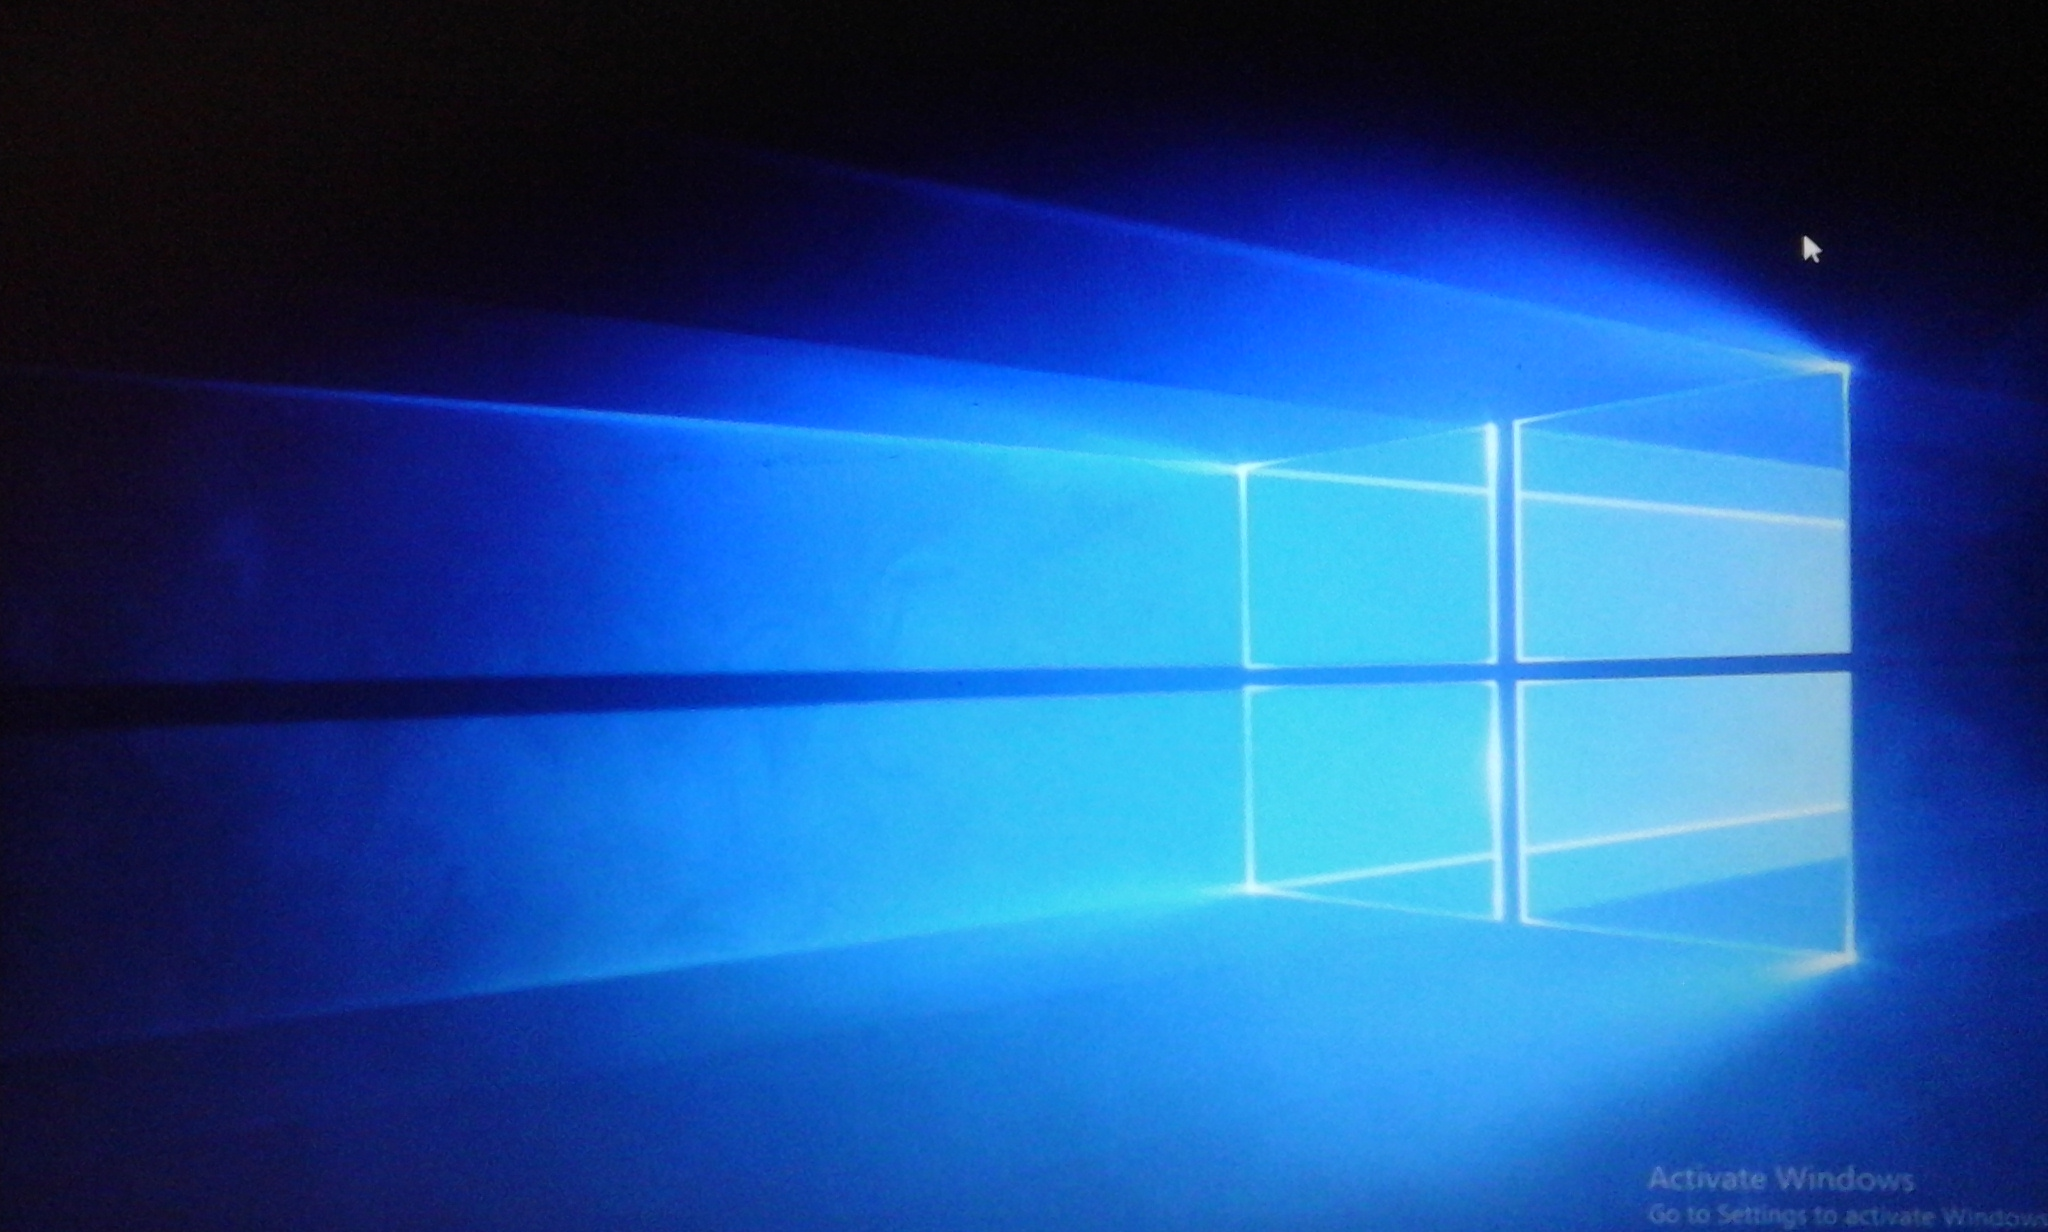
\includegraphics[width=1\textwidth]{figures/tampilanwindows10.JPG}}
\caption{tampilan desktop di windows 10.}
\label{tampilanwindows10}
\end{figure}